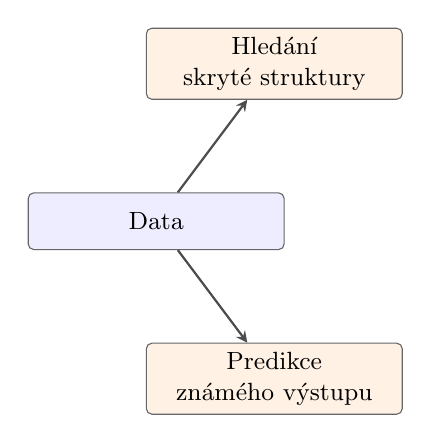
\begin{tikzpicture}[
    >=stealth,
    box/.style={
        draw=black!60,
        rounded corners=2pt,
        align=center,
        font=\small,
        minimum width=3.25cm,
        minimum height=0.72cm
    },
    main/.style={box, fill=blue!7},
    branch/.style={box, fill=orange!10},
    arr/.style={->, thick, draw=black!70}
]
    \node[main] (data) {Data};
    \node[branch] (pred) at (1.5,-2.0) {Predikce\\známého výstupu};
    \node[branch] (struct) at (1.5,2.0) {Hledání\\skryté struktury};

    \draw[arr] (data) -- (pred);
    \draw[arr] (data) -- (struct);
\end{tikzpicture}
